%---------------------------------------------------------------------------------------------------------------------------
% Kopf des Vortrags
%---------------------------------------------------------------------------------------------------------------------------

\part{Sensordatenfusion}
\begin{center}
Janfabian Fabriczek, \\ Geschwister-Scholl-Stra�e 15, 73732 Esslingen,\\ E-Mail: janfabian.fabriczek@stud.hs-esslingen.de \\[1cm] 01. April 2019 \\[1cm]
\end{center}


%---------------------------------------------------------------------------------------------------------------------------
% Textteil
%---------------------------------------------------------------------------------------------------------------------------
\section*{Einleitung}
\label{Kap_Einleitung}

Das autonome Fahren hat f�r die Automobilbranche einen hohen Stellenwert. Ein Computer steuert das Auto ohne menschlichen Einfluss. Damit der Computer im Auto genau wei� wie, wann und wo es fahren kann und muss, muss es die Umgebung wahrnehmen k�nnen.

Um die Umgebung wahrnehmen zu k�nnen, werden Sensoren am Auto verwendet. In der Au�enwelt gibt es viele verschiedene Wetterbedingungen, die die Sensoren so stark beeinflussen k�nnen, dass sie ihren Zweck nicht mehr erf�llen k�nnen. Der Einsatz mehrerer Sensoren mit unterschiedlichen Wahrnehmungsverfahren hilft, die Blindheit des Autos abzuwehren und somit auch die Sicherheit neben der Funktionsf�higkeit zu erhalten.

Der Einsatz von mehreren Sensoren erfordert allerdings, dass die Messdaten zusammengefasst werden und dadurch ein komplettes Abbild der Umgebung entsteht. Unter dem Begriff \textit{Sensordatenfusion} wird das Zusammenf�hren der Sensordaten verstanden.


%%%%%%%%%%%%%%%%%%%%%%%%%%%%%%%%%%%%%%%%%%%%%%%%%%%%%%%%%%%%%%%%%%%%%%%%%%%%%%%

%\newpage
\section*{Funktionsweise}

\subsection*{Aufbau}

\subsubsection*{Allgemein}

Quisque sed luctus orci. Nam sodales massa ante, eget lacinia sapien mattis eu. Donec turpis

%+++++++++++++++++++++++++++++++++++++++++++++++++++++++++++++
\begin{figure}[ht]
 \centerline{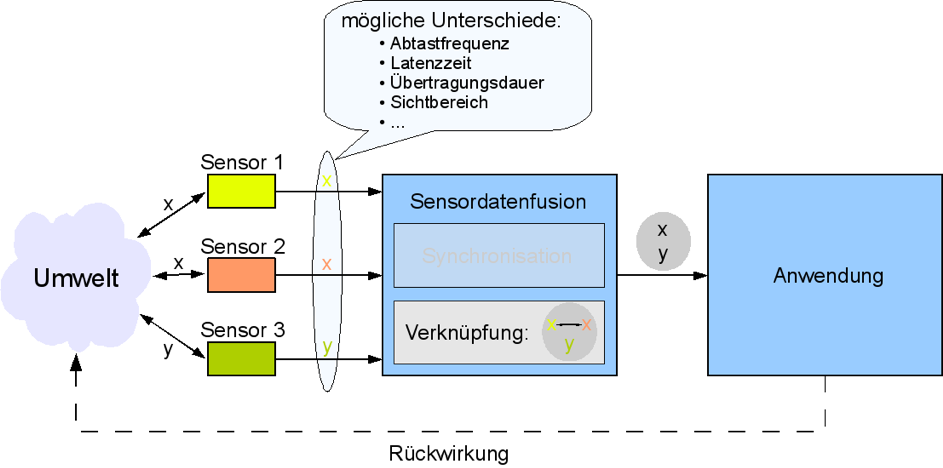
\includegraphics[width=0.41\textwidth]{Name_JFBR/aufbau_allgemein.png}}
 \caption {Condimentum laoreet, lacus nisl pretium}
 \label{Abb_Zustandsraum} 
\end{figure}
%+++++++++++++++++++++++++++++++++++++++++++++++++++++++++++++


\subsubsection*{Sensoren}

Unter einem Sensornetzwerk wird der Verbund mehrerer gleicher oder auch unterschiedlicher Sensoren in einem Netzwerk verstanden.

Die Sensornetzwerke werden zwischen zwei Typen unterschieden. Der eine Typ ist das homogene Sensornetzwerk und der andere Typ ist das heterogene Sensornetzwerk. In einem homogenen Sensornetzwerk verwenden alle Sensoren dasselbe physikalische Prinzip zum Messen. Die Sensoren in einem solchen Netzwerk unterliegen somit alle den gleichen Einschr�nkungen. In einem heterogenen Sensornetzwerk


%%%%%%%%%%%%%%%%%%%%%%%%%%%%%%%%%%%%%%%%%%%%%%%%%%%%%%%%%%%%%%%%%%%%%%%%%%%%%%%

%\newpage
\subsection*{Fusionstyp}

Nullam eu fringilla libero, vel tristique enim. Quisque efficitur ut nunc vel facilisis. Morbi 

\subsubsection*{Across Sensors - Data Fusion}

Nunc pellentesque lacinia metus vehicula auctor. In congue purus diam, vel sollicitudin sapien 

\subsubsection*{Across Attributes - Feature Fusion}

Ut vehicula ultricies maximus. Morbi lacus quam, tincidunt at interdum in, aliquet tempus sem. 

\subsubsection*{Across Domains - Decision Fusion}

Donec venenatis eleifend turpis in mollis. Praesent id mi quis justo feugiat viverra. Sed 

\subsubsection*{Across Time}

Donec mi eros, laoreet sit amet libero eget, laoreet tempus eros. Nulla aliquet nulla nec nibh 


%%%%%%%%%%%%%%%%%%%%%%%%%%%%%%%%%%%%%%%%%%%%%%%%%%%%%%%%%%%%%%%%%%%%%%%%%%%%%%%

%\newpage
\subsection*{Methodik}


%%%%%%%%%%%%%%%%%%%%%%%%%%%%%%%%%%%%%%%%%%%%%%%%%%%%%%%%%%%%%%%%%%%%%%%%%%%%%%%

%\newpage
\section*{Sensorkonfiguration}

Bei der Fusion wird zwischen verschiedenen Typen unterschieden.

\begin{itemize}
\item Redundante oder kompetitive Fusion
\item Komplement�re Fusion
\item Kooperative Fusion
\item Unabh�ngige Fusion
\end{itemize}

\subsection*{Redundant und kompetitiv}

Bei der redundanten oder auch kompetitiven Fusion geschieht die Sammlung der Daten zur Fusion durch den Einsatz mehrerer identischer Sensoren mit demselben Erfassungsbereich, die in einem Sensornetzwerk zusammengef�gt sind.

Da alle eingesetzten Sensoren denselben Erfassungsbereich haben, erh�ht sich durch diesen Fusionstyp nicht der Gesamterfassungsbereich.

Das Ziel dieses Fusionstypen ist die Erh�hung der Genauigkeit der Beobachtung und die Verbesserung der Ausfallsicherheit. Die Erh�hung der Genauigkeit resultiert durch die weiteren Sensoren, die durch das Sensornetzwerk der Fusion zur Verf�gung stehen, die weitere Messwerte erfassen. Die Ausfallsicherheit verbessert sich, da mehrere Sensoren denselben Bereich erfassen und somit der Bereich auch dann noch erfasst wird, wenn mehrere Sensoren ausfallen. 


\subsection*{Komplement�r}

Pellentesque eget turpis quam. Integer varius ante id felis tincidunt, in pharetra lorem laoreet. 

\subsection*{Kooperativ}

Aenean mollis tortor malesuada metus tincidunt tempor. Quisque quis orci nec quam lacinia 

Donec mi eros, laoreet sit amet libero eget, laoreet tempus eros. Nulla aliquet nulla nec nibh 

%+++++++++++++++++++++++++++++++++++++++++++++++++++++++++++++
\begin{figure}[ht]
 \centerline{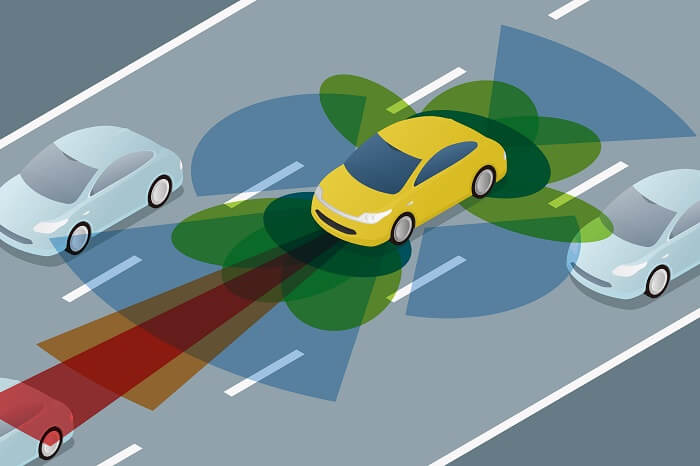
\includegraphics[width=0.41\textwidth]{Name_JFBR/car_sensors.jpg}}
 \caption {Condimentum laoreet, lacus nisl pretium}
 \label{Abb_Zustandsraum} 
\end{figure}
%+++++++++++++++++++++++++++++++++++++++++++++++++++++++++++++

%%%%%%%%%%%%%%%%%%%%%%%%%%%%%%%%%%%%%%%%%%%%%%%%%%%%%%%%%%%%%%%%%%%%%%%%%%%%%%%

%\newpage
\section*{Vorteile}

Als erstes wird der Nachteil ausgeglichen, dass normalerweise nur ein Sensor verwendet wird. Bei der Sensordatenfusion werden mehrere Sensoren eingesetzt. Dies hat den Vorteil, dass die Sch�tzgenauigkeit verbessert wird. Des Weiteren wird der Gesamterfassungsbereich durch den Einsatz von mehreren Sensoren vergr��ert. 
Dar�ber hinaus wird auch eine Verbesserung der Ausfallsicherheit erreicht. Dadurch d�rfen einzelne Sensoren auch ausfallen, ohne dass sie die Funktionsf�higkeit einschr�nken. Aber durch den Ausfall von Sensoren bei der Sensordatenfusion kann sich die durch die Sensordatenfusion verbesserte Sch�tzgenauigkeit und Robustheit wieder verschlechtern. Auch die gewonnene Robustheit des Gesamtsystems kann sich durch den Ausfall mehrere Sensoren verschlechtern, da unter Umst�nden Sensoren ausfallen, die unter bestimmten Umweltbedingungen besser arbeiten, als andere. Um die Ausfallsicherheit nicht zu gef�hrden, werden die Sensoren mit Redundanz ausgelegt. Es bedeutet, dass Sensoren, die zwingend erforderlich f�r die Sicherheit oder die Funktionsf�higkeit sind, mehrfach im Sensornetzwerk eingebunden werden.

Durch den Einsatz von mehreren Sensoren, die unterschiedliche Wahrnehmungsverfahren verwenden, beispielsweise Radar und Laserabstandssensoren, k�nnen die unterschiedlichen St�rken der Wahrnehmungsverfahren zusammengef�hrt werden und verbessern die Wahrnehmung des Erfassungsbereichs. Die Nachteile einzelner Wahrnehmungsverfahren der Sensoren, die unter bestimmten Umweltbedingungen entstehen k�nnen, werden ausgeglichen, da die Wahrnehmung in solchen F�llen beispielsweise haupts�chlich durch einen oder mehrere andere Sensoren �bernommen wird. Die F�higkeit die Umgebung ausreichend zu erfassen, wird somit auch in f�r einzelne Sensoren schwierigen Situationen gew�hrleistet.


%%%%%%%%%%%%%%%%%%%%%%%%%%%%%%%%%%%%%%%%%%%%%%%%%%%%%%%%%%%%%%%%%%%%%%%%%%%%%%%

%\newpage
\section*{Nachteile}

Donec mi eros, laoreet sit amet libero eget, laoreet tempus eros. Nulla aliquet nulla nec nibh 

%%%%%%%%%%%%%%%%%%%%%%%%%%%%%%%%%%%%%%%%%%%%%%%%%%%%%%%%%%%%%%%%%%%%%%%%%%%%%%%

%\newpage
\section*{Einsatzgebiete}
Donec mi eros, laoreet sit amet libero eget, laoreet tempus eros. Nulla aliquet nulla nec nibh 

%%%%%%%%%%%%%%%%%%%%%%%%%%%%%%%%%%%%%%%%%%%%%%%%%%%%%%%%%%%%%%%%%%%%%%%%%%%%%%%
%\newpage

%------------------------------------------------------------------------------------------------------------------------
\section*{Zusammenfassung}

Cras sagittis, ligula quis condimentum laoreet, lacus nisl pretium ligula, sed rutrum ipsum erat in dui. Nam hendrerit velit in dui laoreet, sed eleifend libero commodo. Vivamus pharetra lacus ac viverra hendrerit. Pellentesque dignissim tempus tempor. Nullam sit amet justo libero.

%%%%%%%%%%%%%%%%%%%%%%%%%%%%%%%%%%%%%%%%%%%%%%%%%%%%%%%%%%%%%%%%%%%%%%%%%%%%%%%

\begin{thebibliography}{}

\bibitem{Ref_PGN07}
Wikipedia, Online Nachschlagewerk: \textit{"'Primary Guidance, Navigation and Control System"'},\\  \href{http://de.wikipedia.org/wiki/Primary\_Guidance\%2C\_Navigation\_and\_Control\_System}{http://de.wikipedia.org/wiki/Primary\_Guidance\\\%2C\_Navigation \_and\_Control\_System}, Okt. 2007

\bibitem{Ref_WEN00}
Wenzel, L.: \textit{"'Kalman-Filter - Ein mathematisches Modell zur Auswertung von Messdaten f�r Regelungstechnik, Teil 1"'}, Elektronik 6/2000

\bibitem{Ref_Matrix2008}
Petersen, K. B., Petersen, M. S.: \textit{"'The Matrix Cookbook"'}, http://matrixcookbook.com, Version: November 14, 2008

\bibitem{Ref_Bronstein}
Bronstein, I. N., Semendjajew, K. A.: \textit{"'Taschenbuch der Mathematik"'}, 25. Auflage, Verlag Nauka, Moskau, B.G. Teubner Verlagsgesellschaft Stuttgart, Leipzig, Verlag Harri Deutsch Thun und Frankfurt/Main, 1991

\bibitem{Ref_Kalman1960}
Kalman, R. E.: \textit{"'A New Approach to Linear Filtering and Prediction Problems"'}, Transaction of the ASME, Journal of Basic Engineering, Seiten 35-45, 1960

\bibitem{Ref_GRE01}
Grewal, M. S. und Andrews, P. A.: \textit{"'Kalman filtering: theory and practice using Matlab"'}, second edition, Wiley-Interscience Publication, New York, 2001

\end{thebibliography}

